\Chapter{\readyforreading{Reification by Parametricity}: Fast Setup for Proof by Reflection, in Two Lines of \Ltac}\label{ch:reification-by-parametricity}

%\setlength{\belowdisplayskip}{5pt}% \setlength{\belowdisplayshortskip}{0pt}%
%\setlength{\abovedisplayskip}{5pt}% \setlength{\abovedisplayshortskip}{0pt}%

\section{Introduction} \label{sec:reification-by-parametricity:intro}

We introduced reification in \autoref{sec:reif-intro} as the starting point for proof by reflection.
Reification consists of translating a ``native'' term of the logic into an explicit abstract syntax tree, which we may then feed to verified procedures or any other functional programs in the logic.
As mentioned in \autoref{sec:reif-not-optimized}, the method of reification used in our framework for reflective partial evaluation and rewriting presented in \autoref{ch:rewriting} was not especially optimized and can be a bottleneck for large terms, especially those with many binders.
Popular methods turn out to be surprisingly slow, often to the point where, counterintuitively, the majority of proof-execution time is spent in reification -- unless the proof engineer invests in writing a plugin directly in the proof assistant's metalanguage (e.g., OCaml for Coq).

In this chapter, we present a new strategy we discovered during my doctoral work, originally presented and published as \cite{reification-by-parametricity}, showing that reification can be both simpler and faster than with standard methods.
\todoac{about the previous sentence: These three pronouns are inconsistent. Your coauthors are not presenting the results *here*.}
Perhaps surprisingly, we demonstrate how to reify terms almost entirely through reduction in the logic, with a small amount of tactic code for setup and no ML programming.
%Though our techniques should be broadly applicable, especially in proof assistants based on type theory, our experience is with Coq
We have already summarized our survey into prior approaches to reification \autoref{sec:reif-survey}, providing high-quality implementations and documentation for them, serving a tutorial function independent of our new contributions.
We will begin in \autoref{sec:reification-by-parametricity} with an explanation of our alternative technique.
We benchmark our approach against 18 competitors in \autoref{sec:perf}.

\section{Reification by Parametricity}\label{sec:reification-by-parametricity}

We propose factoring reification into two passes, both of which essentially have robust, built-in implementations in Coq: \emph{abstraction} or \emph{generalization}, and \emph{substitution} or \emph{specialization}.


\begin{wrapfigure}[10]{r}{7.25cm}
%    \vspace{-40pt}
    \[
    \xymatrix{
        \txt{term}
        \ar@<1ex>[ddr]|-{\txt{\rotatebox{-40}{generalize}}}
        \ar@<-1ex>@{-->}[rr]_{\txt{reify}}
        &&
        \txt{reified \\ syntax}
        \ar@<-1ex>[ll]_{\txt{denote}}
        \ar@<-1ex>[ddl]|-{\txt{\rotatebox{40}{generalize}}}
        \\ \\
        &
        \txt{abstracted term}
        \ar@<1ex>[uul]|-{\txt{\rotatebox{-40}{specialize}}}
        \ar@<-1ex>[uur]|-{\txt{\rotatebox{40}{specialize}}}
    }
    \]
%    \vspace{-20pt}
    \caption{Abstraction and Reification}\label{fig:denote-reify}
\end{wrapfigure}

The key insight to this factoring is that the shape of a reified term is essentially the same as the shape of the term that we start with.
We can make precise the way these shapes are the same by abstracting over the parts that are different, obtaining a function that can be specialized to give either the original term or the reified term.

That is, we have the commutative triangle in \autoref{fig:denote-reify}.

\subsection{Case-By-Case Walkthrough} \label{sec:case-by-case-walkthrough}
\subsubsection{Function Applications and Constants.} \label{sec:reification-by-parametricity-diagram}\label{sec:walkthrough-func-const}
Consider the example of reifying $2\times 2$.
In this case, the \emph{term} is $2 \times 2$ or (mul (S (S O)) (S (S O))).

To reify, we first \emph{generalize} or \emph{abstract} the term $2\times 2$ over the successor function S, the zero constructor O, the multiplication function mul, and the type $\mathbb N$ of natural numbers.
We get a function taking one type argument and three value arguments:
$$\Lambda N. \; \lambda (\textsc{Mul} : N \to N \to N) \; (\text{O} : N) \; (\text{S} : N \to N). \; \text{\textsc{Mul} (S (S O)) (S (S O))}$$

We can now specialize this term in one of two ways: we may substitute $\mathbb N$, mul, O, and S, to get back the term we started with; or we may substitute \texttt{expr}, \texttt{NatMul}, \texttt{NatO}, and \texttt{NatS} to get the reified syntax tree
\[
\texttt{NatMul (NatS (NatS NatO)) (NatS (NatS NatO))}
\]

This simple two-step process is the core of our algorithm for reification:
abstract over all identifiers (and key parts of their types) and specialize to syntax-tree constructors for these identifiers.

\subsubsection{Wrapped Primitives: \texorpdfstring{\mintinline{coq}{let}}{let} Binders, Eliminators, Quantifiers.}\label{sec:walkthrough-wrapped}

The above procedure can be applied to a term that contains \mintinline{coq}{let} binders to get a
PHOAS tree that represents the original term, but doing so would not capture
sharing. The result would contain native \mintinline{coq}{let} bindings of subexpressions, not
PHOAS let expressions. Call-by-value evaluation of any procedure applied to the
reification result would first substitute the let-bound subexpressions --
leading to potentially exponential blowup and, in practice, memory exhaustion.

The abstraction mechanisms in all proof assistants (that we know about) only allow abstracting over terms, not language primitives.
However, primitives can often be wrapped in explicit definitions, which we \emph{can} abstract over.
For example, we already used a wrapper for \mintinline{coq}{let} binders, and terms that use it can be reified by abstracting over that definition.
If we start with the expression
\[
\text{\texttt{dlet} }a := 1\texttt{ in }a \times a
\]
and abstract over $(\texttt{@Let\_In $\mathbb N$ $\mathbb N$})$, S, O, mul, and $\mathbb{N}$,
we get a function of one type argument and four value arguments:
\begin{multline*}
\Lambda N.\,\lambda
\ (\textsc{Mul} : N \to N \to N).
\ \lambda (\text{O} : N).
\ \lambda (\text{S} : N \to N). \\
\ \lambda (\textsc{LetIn} : N \to (N\to N)\to N).
\ \textsc{LetIn (S O) ($\lambda a.$ Mul $a$ $a$)}
\end{multline*}
We may once again specialize this term to obtain either our original term or the reified syntax.
Note that to obtain reified PHOAS, we must include a \texttt{Var} node in the \texttt{LetIn} expression; we substitute $(\lambda x\ f.\ \texttt{LetIn}\ x\ (\lambda v.\ f\ (\texttt{Var}\ v)))$ for \textsc{LetIn} to obtain the PHOAS tree
\[
  \texttt{LetIn (NatS NatO) ($\lambda v.$ NatMul (Var $v$) (Var $v$))}
\]

Wrapping a metalanguage primitive in a definition in the code to be reified is in general sufficient for reification by parametricity.
Pattern matching and recursion cannot be abstracted over directly, but if the same code is expressed using eliminators, these can be handled like other functions.
Similarly, even though $\forall$/$\Pi$ cannot be abstracted over, proof automation that itself introduces universal quantifiers before reification can easily wrap them in a marker definition (\texttt{\_forall T P := forall (x:T), P x}) that can be.
Existential quantifiers are not primitive in Coq and can be reified directly.

\subsubsection{Lambdas.}\label{sec:walkthrough-lambdas}

While it would be sufficient to require that, in code to be reified, we write all lambdas with a named wrapper function, that would significantly clutter the code.
We can do better by making use of the fact that a PHOAS object-language lambda (\texttt{Abs} node) consists of a metalanguage lambda that binds a value of type \texttt{var}, which can be used in expressions through constructor $\mathtt{Var} : \mathtt{var} \to \mathtt{expr}$.
Naïve reification by parametricity would turn a lambda of type $N \to N$ into a lambda of type $\mathtt{expr} \to \mathtt{expr}$.
A reification procedure that explicitly recurses over the metalanguage syntax could just precompose this recursive-call result with \texttt{Var} to get the desired object-language encoding of the lambda, but handling lambdas specially does not fit in the framework of abstraction and specialization.

First, let us handle the common case of lambdas that appear as arguments to higher-order functions.
One easy approach: while the parametricity-based framework does not allow for special-casing lambdas, it is up to us to choose how to handle functions that we expect will take lambdas as arguments.
We may replace each higher-order function with a metalanguage lambda that wraps the higher-order arguments in object-language lambdas, inserting \texttt{Var} nodes as appropriate.
Code calling the function $\text{\texttt{sum\_upto} }n\; f := f(0) + f(1) + \cdots + f(n)$ can be reified by abstracting over relevant definitions and substituting
$(\lambda n\ f.\ \texttt{SumUpTo}\ n\ (\texttt{Abs}\ (\lambda v.\ f\ (\texttt{Var}\ v))))$ for $\text{\texttt{sum\_upto}}$.
Note that the expression plugged in for \texttt{sum\_upto} differs from the one plugged in for \texttt{Let\_In} only in the use of a deeply embedded abstraction node.
If we wanted to reify \texttt{LetIn} as just another higher-order function (as opposed to a distinguished wrapper for a primitive), the code would look identical to that for \texttt{sum\_upto}.

It would be convenient if abstracting and substituting for functions that take higher-order arguments were enough to reify lambdas, but here is a counterexample.
Starting with
\[
  \lambda\ x\ y.\ x \times ((\lambda\ z.\ z \times z)\ y),
\]
abstraction gives
\[
  \Lambda N. \; \lambda (\textsc{Mul} : N \to N \to N).\ \lambda\ (x\ y : N).\ \texttt{Mul}\ x\ ((\lambda\ (z : N).\ \texttt{Mul}\ z\  z)\ y),
\]
and specialization and reduction give
\[
  \lambda\ (x\ y : \texttt{expr}).\ \texttt{NatMul}\ x\ (\texttt{NatMul}\ y\  y).
\]
The result is not even a PHOAS expression. We claim a desirable reified form is
\[
  \texttt{Abs}(\lambda\ x.\ \texttt{Abs}(\lambda\ y.\ \texttt{NatMul}\ (\texttt{Var}\ x)\ (\texttt{NatMul}\ (\texttt{Var}\ y)\  (\texttt{Var}\ y))))
\]
Admittedly, even our improved form is not quite precise: $\lambda\ z.\, z \times z$ has been lost. However, as almost all standard Coq tactics silently reduce applications of lambdas, working under the assumption that functions not wrapped in definitions will be arbitrarily evaluated during scripting is already the norm.
Accepting that limitation, it remains to consider possible occurrences of metalanguage lambdas in normal forms of outputs of reification as described so far.
As lambdas in \texttt{expr} nodes that take metalanguage functions as arguments (\texttt{LetIn}, \texttt{Abs}) are handled by the rules for these nodes, the remaining lambdas must be exactly at the head of the expression.
Manipulating these is outside of the power of abstraction and specialization; we recommend postprocessing using a simple recursive tactic script.

\subsection{Commuting Abstraction and Reduction} \label{sec:commute-abstraction-reduction}
Sometimes, the term we want to reify is the result of reducing another term.
For example, we might have a function that reduces to a term with a variable number of \texttt{let} binders.\footnote{%
    More realistically, we might have a function that represents big numbers using multiple words of a user-specified width.
    In this case, we may want to specialize the procedure to a couple of different bitwidths, then reify the resulting partially reduced terms.%
}
We might have an inductive type that counts the number of \letindots\space nodes we want in our output.
\label{sec:count-def}
\begin{verbatim}
Inductive count := none | one_more (how_many : count).
\end{verbatim}
It is important that this type be syntactically distinct from $\mathbb N$ for reasons we will see shortly.

\begin{wrapfigure}[5]{r}{8.5cm}
%    \vspace{-33pt}
    \[
    \xymatrix@C=1pt{
        \txt{unreduced term \\ (big $1$ $n$)} \ar[d]_{\txt{\\reduce}} \\
        \txt{reduced \\ term}
        \ar@<1ex>[ddr]|-{\txt{\rotatebox{-45}{generalize}}}
        \ar@<-1ex>@{-->}[rr]_{\txt{reify}}
        &&
        \txt{reified \\ syntax}
        \ar@<-1ex>[ll]_{\txt{denote}}
        \ar@<-1ex>[ddl]|-{\txt{\rotatebox{52}{generalize}}}
        \\ \\
        &
        \txt{abstracted term}
        \ar@<1ex>[uul]|-{\txt{\rotatebox{-45}{specialize}}}
        \ar@<-1ex>[uur]|-{\txt{\rotatebox{52}{specialize}}}
    }
    \]
%    \vspace{-10pt}
    \caption{Abstraction, Reification, Reduction} \label{fig:reduce-denote-reify}
\end{wrapfigure}

We can then define a recursive function that constructs some number of nested \texttt{let} binders:
\label{sec:big-def}
\begin{verbatim}
Fixpoint big (x:nat) (n:count)
  : nat
  := match n with
     | none => x
     | one_more n'
      => dlet x' := x * x in
         big x' n'
     end.
\end{verbatim}
Our commutative diagram in \autoref{fig:denote-reify} now has an additional node, becoming \autoref{fig:reduce-denote-reify}.
Since generalization and specialization are proportional in speed to the size of the term begin handled, we can gain a significant performance boost by performing generalization before reduction.
To explain why, we split apart the commutative diagram a bit more; in reduction, there is a $\delta$ or unfolding step, followed by a $\beta\iota$ step that reduces applications of $\lambda$s and evaluates recursive calls.
In specialization, there is an application step, where the $\lambda$ is applied to arguments, and a $\beta$-reduction step, where the arguments are substituted.
To obtain reified syntax, we may perform generalization after $\delta$-reduction (before $\beta\iota$-reduction), and we are not required to perform the final $\beta$-reduction step of specialization to get a well-typed term.
It is important that unfolding \texttt{big} results in exposing the body for generalization, which we accomplish in Coq by exposing the anonymous recursive function; in other languages, the result may be a primitive eliminator applied to the body of the fixpoint.
Either way, our commutative diagram thus becomes \label{sec:expanded-reif-diagram}
\[
\xymatrix@R=0.5em{
    \txt{unreduced term} \ar[d]^{\delta} \\
    \txt{small partially \\ reduced term}
    \ar[r]^{\beta\iota}
    \ar@<1ex>[ddddrr]
    & \txt{reduced \\ term}
    \ar@<1ex>[ddr]
    \ar@<-1ex>@{-->}[rr]
    &&
    \txt{reduced \\ reified syntax}
    \ar@<-1ex>[ll]
    \ar@<-1ex>[ddl]
    \\ \\
    &&
    \txt{abstracted \\ term}
    \ar@<1ex>[uul]
    \ar@<-1ex>[uur]%|{\text{application; $\beta$-reduction}}
    &
    \txt{unreduced \\ reified syntax}
    \ar@<1ex>[ddl]
    \ar[uu]_{\beta\iota}
    \\ \\
    &&
    \txt{unreduced \\ abstracted term}
    \ar@<1ex>[uuuull]
    \ar@<1ex>[uur]^{\rotatebox{25}{\llap{\text{application\hspace*{-2em}}}}}
}
\]
%\[
%\xymatrix{
%    \txt{unreduced term} \ar[d]^{\delta} \\
%    \txt{small partially \\ reduced term} \ar[r]^{\beta\iota} \ar@/_1pc/[dd]
%    & \txt{reduced term} \ar@/_1pc/[dd] \\
%    &&& \txt{reduced \\ reified syntax}
%    \\
%    \txt{unreduced \\ abstrated term}\ar[r]^{\beta\iota} \ar@/_1pc/[uu] \ar@/_1.5pc/[dr]_{\text{application}}
%    &\txt{abstracted term} \ar@/_1pc/[uu]
%    \ar@/_1.5pc/[urr]|{\text{application; }\beta\text{-reduction}} && \\
%    &\txt{unreduced \\ reified syntax} \ar@/_4pc/[uurr]_{\beta\iota}
%}
%\]
Let us step through this alternative path of reduction using the example of the unreduced term \texttt{big 1 100}, where we take 100 to mean the term represented by $\underbrace{(\texttt{one\_more} \cdots (\texttt{one\_more}}_{100}\  \texttt{none}\underbrace{) \cdots )}_{100}$.

Our first step is to unfold \texttt{big}, rendered as the arrow labeled $\delta$ in the diagram.
In Coq, the result is an anonymous fixpoint; here we will write it using the recursor \texttt{count\_rec} of type $\forall T.\ T \to (\texttt{count} \to T \to T) \to \texttt{count} \to T$.
Performing $\delta$-reduction, that is, unfolding \texttt{big}, gives us the small partially reduced term
\begin{multline*}
\big(\lambda (x:\mathbb N).\ \lambda(n : \texttt{count}). \\
\texttt{count\_rec}\ (\mathbb N \to \mathbb N)\ (\lambda x.\ x)\ (\lambda n'.\ \lambda\texttt{big}_{n'}.\ \lambda x.\ \texttt{dlet }x' := x \times x\texttt{ in } \texttt{big}_{n'}\ x')\big)\ 1\ 100
\end{multline*}

We call this term small, because performing $\beta\iota$ reduction gives us a much larger reduced term:
\begin{align*}
& \texttt{dlet }x_1 := 1 \times 1\texttt{ in } \cdots \texttt{ dlet }x_{100} := x_{99} \times x_{99}\texttt{ in } x_{100}
\end{align*}

Abstracting the small partially reduced term over $(\texttt{@Let\_In $\mathbb N$ $\mathbb N$})$, S, O, mul, and $\mathbb N$ gives us the abstracted unreduced term
\begin{align*}
\Lambda N.\,\lambda & (\textsc{Mul} : N \to N \to N)%.\\
%& \lambda
 (\text{O} : N)%. \\
%& \lambda
 (\text{S} : N \to N)%. \\
%& \lambda
 (\textsc{LetIn} : N \to (N\to N)\to N). \\
& \big(\lambda (x : N).\ \lambda(n : \texttt{count}).\ %\\
%&\phantom{\big(}
\texttt{count\_rec}\ %\\
%&\phantom{\big(\texttt{count}}
(N \to N)\ %\\
%&\phantom{\big(\texttt{count\_rec}\ }
(\lambda x.\ x) \\
&\phantom{\big(\texttt{count}}(\lambda n'.\ \lambda\texttt{big}_{n'}.
  \ \lambda x.
  \ \textsc{LetIn}\ (\textsc{Mul}\ x\ x)\ (\lambda x'.\ \texttt{big}_{n'}\ x'))\big)\\
& (\text{S O})\ \  %\\
%&
 100
\end{align*}

Note that it is essential here that \texttt{count} is not syntactically the same as $\mathbb N$; if they were the same, the abstraction would be ill-typed, as we have not abstracted over \texttt{count\_rec}.
More generally, it is essential that there is a clear separation between types that we reify and types that we do not, and we must reify \emph{all} operations on the types that we reify.

We can now apply this term to \texttt{expr}, \texttt{NatMul}, \texttt{NatS}, \texttt{NatO}, and, finally, to the term $(\lambda v\ f.\ \texttt{LetIn}\ v\ (\lambda x.\ f\ (\texttt{Var}\ x)))$.
We get an unreduced reified syntax tree of type \texttt{expr}.
If we now perform $\beta\iota$ reduction, we get our fully reduced reified term.

We take a moment to emphasize that this technique is not possible with any other method of reification.
We could just as well have not specialized the function to the \texttt{count} of \texttt{100}, yielding a function of type \texttt{count $\to$ expr}, despite the fact that our reflective language knows nothing about \texttt{count}!

This technique is especially useful for terms that will not reduce without concrete parameters but which should be reified for many different parameters.
Running reduction once is slightly faster than running OCaml reification once, and it is more than twice as fast as running reduction followed by OCaml reification.
For sufficiently large terms and sufficiently many parameter values, this performance beats even OCaml reification.%
\footnote{%
    We discovered this method in the process of needing to reify implementations of cryptographic primitives~\cite{FiatCryptoSP19} for a couple hundred different choices of numeric parameters (e.g., prime modulus of arithmetic).
    A couple hundred is enough to beat the overhead.%
}

\subsection{Implementation in \Ltac}

\texttt{ExampleMoreParametricity.v} in the associated codebase, available at \url{https://github.com/mit-plv/reification-by-parametricity}, mirrors the development of reification by parametricity in \autoref{sec:case-by-case-walkthrough}.

Unfortunately, Coq does not have a tactic that performs abstraction.%
\footnote{%
    The \texttt{generalize} tactic returns $\forall$ rather than $\lambda$, and it only works on types.%
}
However, the \texttt{pattern} tactic suffices; it performs abstraction followed by application, making it a sort of one-sided inverse to $\beta$-reduction.
By chaining \texttt{pattern} with an \Ltac-\texttt{match} statement to peel off the application, we can get the abstracted function.
% We can write:
\begin{verbatim}
Ltac Reify x :=
match (eval pattern nat, Nat.mul, S, O, (@Let_In nat nat) in x) with
| ?rx _ _ _ _ _ =>
 constr:( fun var => rx (@expr var) NatMul NatS NatO
                        (fun v f => LetIn v (fun x => f (Var x))) )
end.
\end{verbatim}
Note that if \texttt{@expr var} lives in \texttt{Type} rather than \texttt{Set}, we must \texttt{pattern} over \texttt{(nat : Type)} rather than \texttt{nat}.
In older versions of Coq, an additional step involving retyping the term with the \Ltac\space primitive \texttt{type of} is needed; we refer the reader to \texttt{Parametricity.v} in the code supplement.

The error messages returned by the \texttt{pattern} tactic can be rather opaque at times; in \texttt{ExampleParametricityErrorMessages.v}, we provide a procedure for decoding the error messages.

\subsubsection{Open Terms.}
At some level it is natural to ask about generalizing our method to reify open terms (i.e., with free variables), but we think such phrasing is a red herring.
Any lemma statement about a procedure that acts on a representation of open terms would need to talk about how these terms would be closed.
For example, solvers for algebraic goals without quantifiers treat free variables as implicitly universally quantified.
The encodings are invariably ad-hoc: the free variables might be assigned unique numbers during reification, and the lemma statement would be quantified over a sufficiently long list that these numbers will be used to index into.
Instead, we recommend directly reifying the natural encoding of the goal as interpreted by the solver, e.g. by adding new explicit quantifiers.
Here is a hypothetical goal and a tactic script for this strategy:
\[
  \texttt{(a b : nat) (H : 0 < b) |- ∃ q r, a = q × b + r ∧ r < b}
\]
\begin{verbatim}
repeat match goal with
       | n : nat |- ?P =>
         match eval pattern n in P with
         | ?P' _ => revert n; change (_forall nat P')
         end
       | H : ?A  |- ?B => revert H; change (impl A B)
       | |- ?G => (* ∀ a b, 0 < b -> ∃ q r, a = q × b + r ∧ r < b *)
         let rG := Reify G in
         refine (nonlinear_integer_solver_sound rG _ _);
         [ prove_wf | vm_compute; reflexivity ]
       end.
\end{verbatim}

Briefly, this script replaced the context variables \texttt{a} and \texttt{b} with universal quantifiers in the conclusion, and it replaced the premise \texttt{H} with an implication in the conclusion.
The syntax-tree datatype used in this example can be found in the Coq source file \texttt{ExampleMoreParametricity.v}.

\subsection{Advantages and Disadvantages}
This method is faster than all but \LtacTwo\space and OCaml reification, and commuting reduction and abstraction makes this method faster even than the low-level \LtacTwo\space reification in many cases.
Additionally, this method is much more concise than nearly every other method we have examined, and it is very simple to implement.
%Unlike every other method of reification, reification by parametricity does not require us to start from reduced terms, where every term that appears is one that we can handle.
%We will come back to this point shortly.

%\subsection{Limitations and Usefulness} \label{sec:limitations-and-strengths}
We will emphasize here that this strategy shines when the initial term is small, the partially computed terms are big (and there are many of them), and the operations to evaluate are mostly well-separated by types (e.g., evaluate all of the \texttt{count} operations and none of the \texttt{nat} ones).

%Although this strategy allows fusing partial evaluation with reification, it does not work if the term needs CPS conversion before partial evaluation, and the method is somewhat painful (but workable) if the term is already CPS-converted and involves higher-order or type-level quantification.
%It only works if the precise application-node structure of the term is not important; if every application node (or \texttt{match} or \letindots) needs to show up in the syntax tree, our approach is not a good match.
This strategy is not directly applicable for reification of \texttt{match} (rather than eliminators) or \letindots\space (rather than a definition that unfolds to \letindots), \texttt{forall} (rather than a definition that unfolds to \texttt{forall}), or when reification should not be modulo $\beta\iota\zeta$-reduction.

\section{Performance Comparison} \label{sec:perf}
We have done a performance comparison of the various methods of reification to the PHOAS language \texttt{@expr var} from \autoref{sec:phoas-expr-def} in Coq 8.12.2.
A typical reification routine will obtain the term to be reified from the goal, reify it, run \texttt{transitivity (denote reified\_term)} (possibly after normalizing the reified term), and solve the side condition with something like \texttt{lazy [denote]; reflexivity}.
Our testing on a few samples indicated that using \texttt{change} rather than \texttt{transitivity; lazy [denote]; reflexivity} can be around 3X slower; note that we do not test the time of \texttt{Defined}.

There are two interesting metrics to consider:
(1) how long does it take to reify the term?
and (2) how long does it take to get a normalized reified term, i.e., how long does it take both to reify the term and normalize the reified term?
We have chosen to consider (1), because it provides the most fine-grained analysis of the actual reification method.

\subsection{Without Binders} \label{sec:perf:no-binders}
We look at terms of the form \texttt{1 * 1 * 1 * \ldots} where multiplication is associated to create a balanced binary tree.
We say that the \emph{size of the term} is the number of $1$s.
We refer the reader to the attached code for the exact test cases and the code of each reification method being tested.

We found that the performance of all methods is linear in term size.

\begin{figure}
\noindent 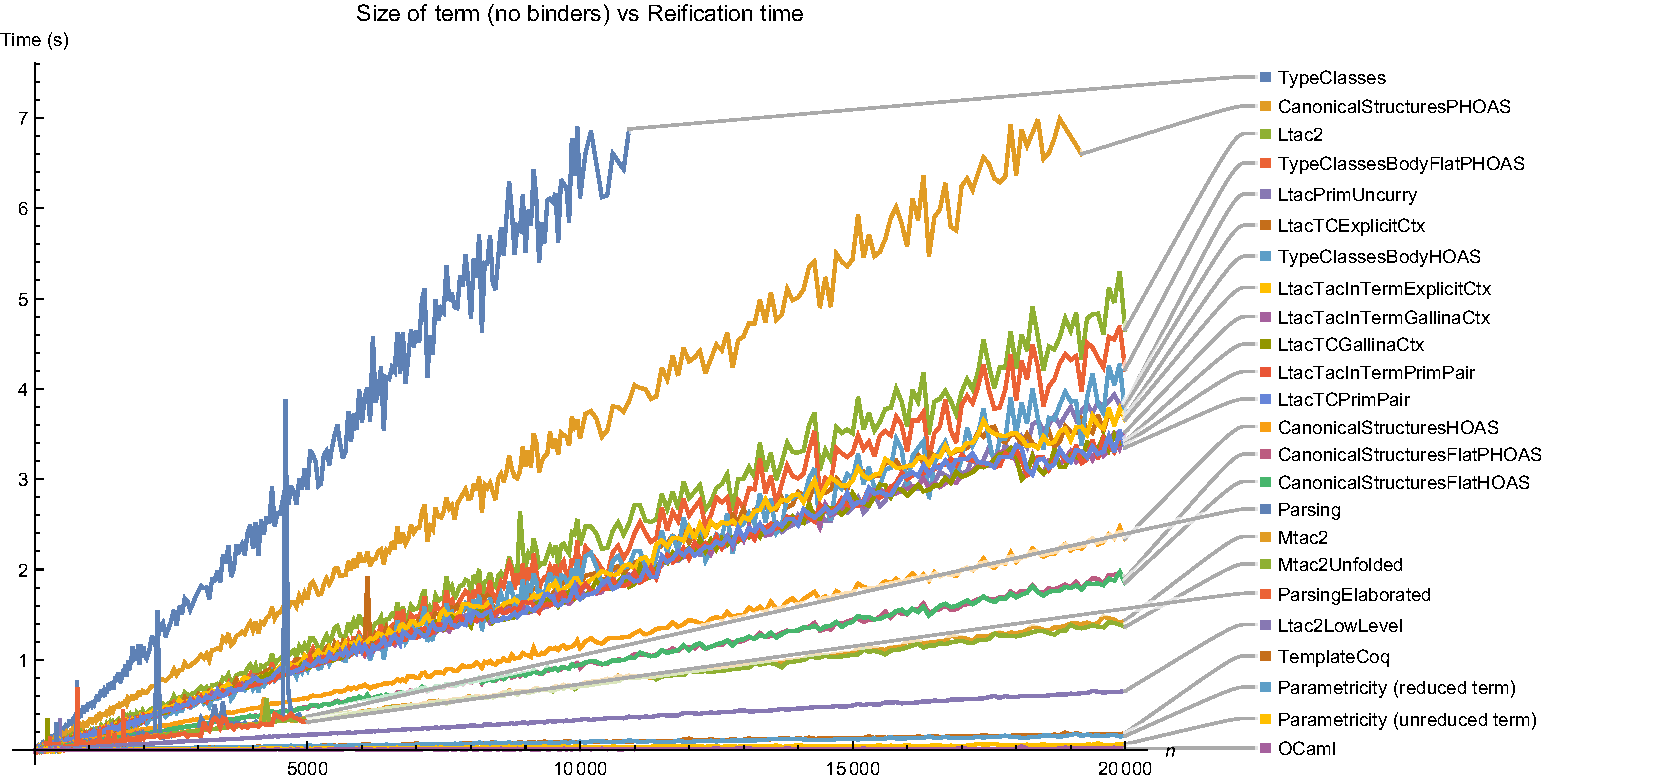
\includegraphics[width=\textwidth]{reification-by-parametricity-outputs/actual-reif-no-binders.pdf}
\caption{Performance of Reification without Binders}\label{fig:graph-reif-no-binders}
\end{figure}

Sorted from slowest to fastest, most of the labels in \autoref{fig:graph-reif-no-binders} should be self-explanatory and are found in similarly named \texttt{.v} files in the associated code; we call out a few potentially confusing ones:
\begin{itemize}
  \item
    The ``Parsing'' benchmark is ``reification by copy-paste'': a script generates a \texttt{.v} file with notation for an already-reified term; we benchmark the amount of time it takes to parse and typecheck that term.
    The ``ParsingElaborated'' benchmark is similar, but instead of giving notation for an already-reified term, we give the complete syntax tree, including arguments normally left implicit.
    Note that these benchmarks cut off at around 5000 rather than at around 20\,000, because on large terms, Coq crashes with a stack overflow in parsing.
    %For size reasons, we do not include these \texttt{.v} files in the associated code tarball, but they can be made via the \texttt{parsing-test-files} target, which generates some files in \texttt{Benchmarks/}.
%  \item
%    In \autoref{sec:ltac2-reif} we mention both a naïve transcription of \Ltac1 to \Ltac2 and a procedure using low-level primitives in \Ltac2; ``Ltac2'' benchmarks the former, and ``Ltac2LowLevel'' benchmarks the latter.
  \item
    We have four variants starting with ``CanonicalStructures'' here.
    The Flat variants reify to \texttt{@expr nat} rather than to \texttt{forall var, @expr var} and benefit from fewer function binders and application nodes.
    The HOAS variants do not include a case for \letindots\space nodes, while the PHOAS variants do.
    Unlike most other reification methods, there is a significant cost associated with handling more sorts of identifiers in canonical structures.
\end{itemize}

We note that on this benchmark our method is slightly faster than template-coq, which reifies to de Bruijn indices, and slightly slower than the quote plugin in the standard library\footnote{This plugin no longer appears in this graph because it was removed in Coq 8.10~\cite{coq-pr-remove-quote-plugin}, though it appears in the graph in \textcite{reification-by-parametricity}.} and the OCaml plugin we wrote by hand.

\subsection{With Binders} \label{sec:perf:binders}

We look at terms of the form \texttt{dlet a$_1$ := 1 * 1 in dlet a$_2$ := a$_1$ * a$_1$ in \ldots\space dlet a$_n$ := a$_{n-1}$ * a$_{n-1}$ in a$_n$}, where $n$ is the size of the term.
The first graph shown here includes all of the reification variants at linear scale, while the next step zooms in on the highest-performance variants at log-log scale.

\begin{figure}[t]
\noindent 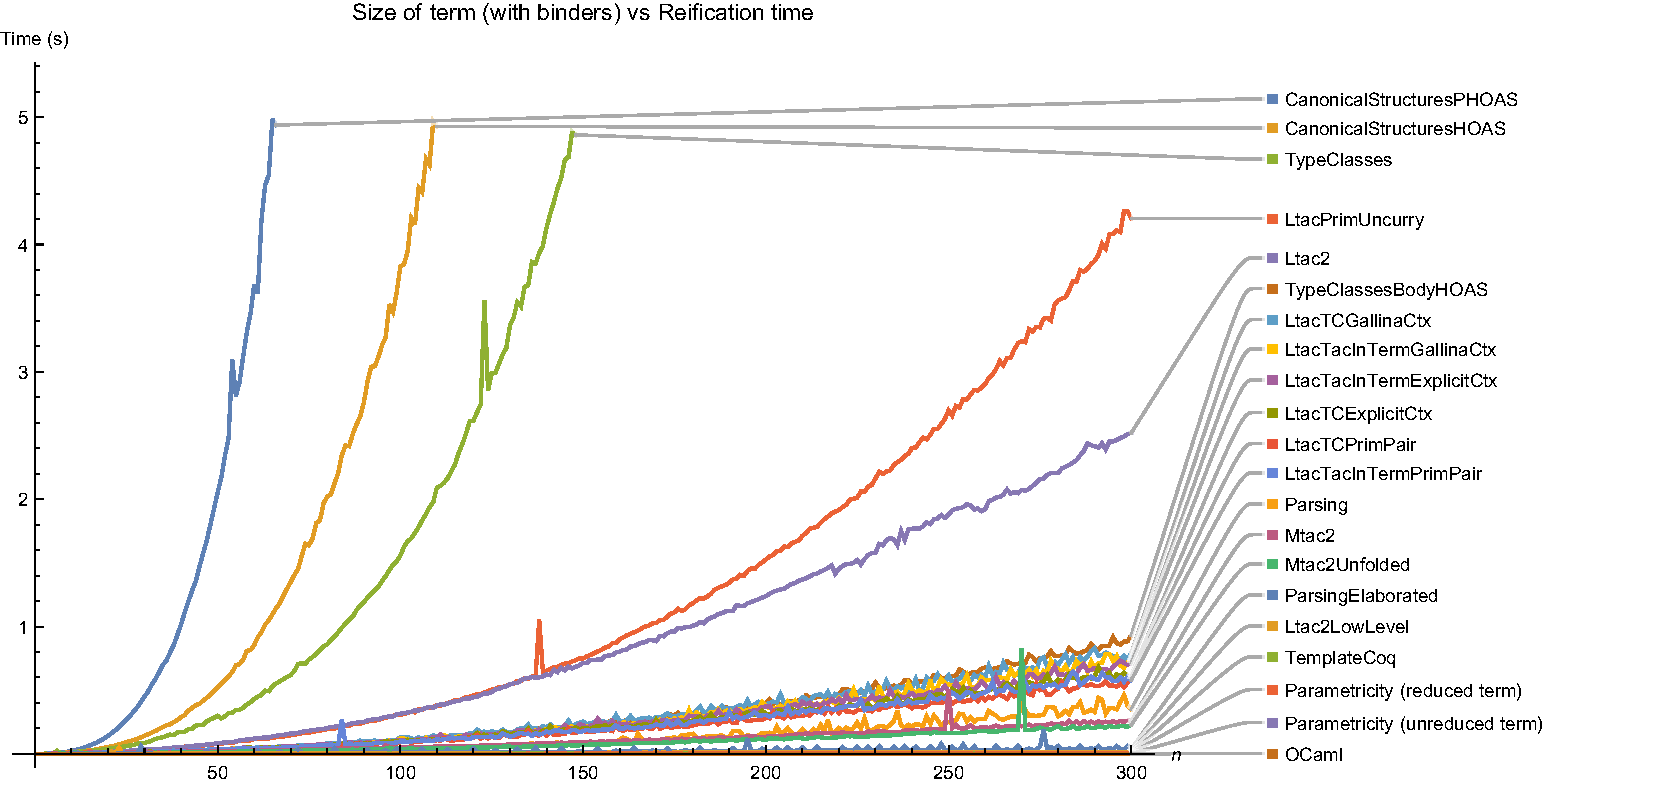
\includegraphics[width=\textwidth]{reification-by-parametricity-outputs/actual-reif-with-binders.pdf}

\noindent 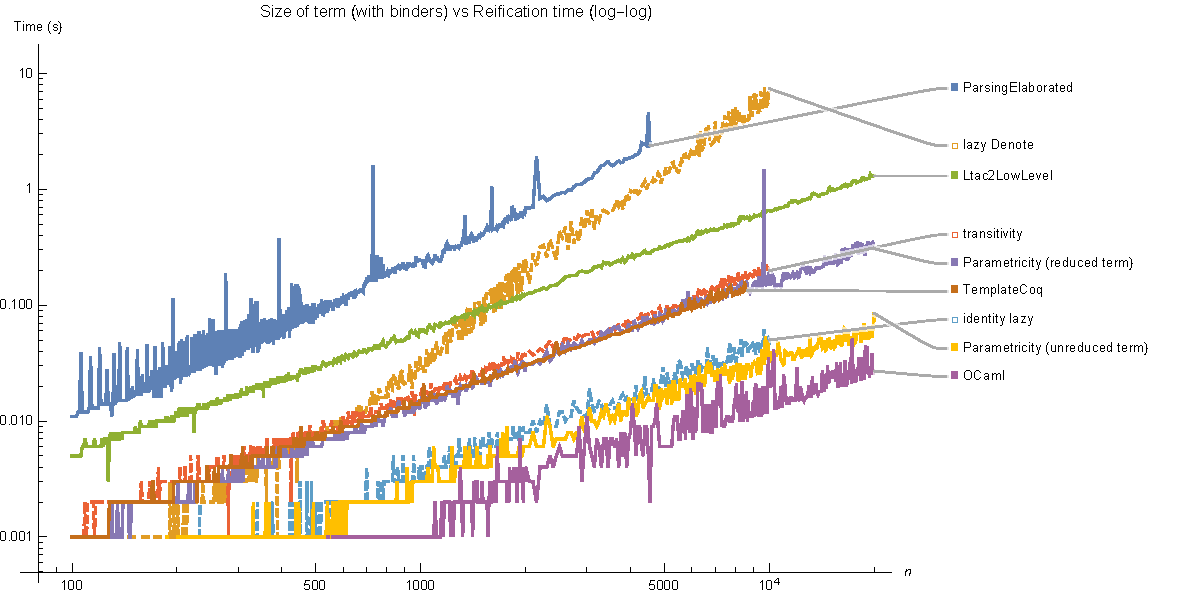
\includegraphics[width=\textwidth]{reification-by-parametricity-outputs/actual-reif-with-binders-log-log-subset.pdf}
\caption{Performance of Reification with Binders}\label{fig:reif-binders}
\end{figure}

In addition to reification benchmarks, the graph in \autoref{fig:reif-binders} includes as a reference (1) the time it takes to run \texttt{lazy} reduction on a reified term already in normal form (``identity lazy'') and (2) the time it takes to check that the reified term matches the original native term (``lazy Denote'').
The former is just barely faster than OCaml reification; the latter often takes longer than reification itself.
The line for the template-coq plugin cuts off at around 10\,000 rather than around 20\,000 because at that point template-coq starts crashing with stack overflows.

\section{Future Work, Concluding Remarks} \label{sec:future}

We identify one remaining open question with this method that has the potential of removing the next largest bottleneck in reification: using reduction to show that the reified term is correct.

\begin{wrapfigure}[11]{r}{9cm}
%\vspace{-36pt}
\[
\xymatrix@R=0.5em@C=0em{
    \txt{unreduced term} \ar[d]^{\delta} \\
    \txt{small partially \\ reduced term}
    \ar@<1ex>[ddr]
    \ar@<-1ex>@{--}[rr]
    &&
    \txt{unreduced \\ reified syntax}
    \ar@<-1ex>@{--}[ll]^{???}
    \ar@<1ex>[ddl]
    \\ \\
    &
    \txt{unreduced \\ abstracted term}
    \ar@<1ex>[uul]
    \ar@<1ex>[uur]%^{\rotatebox{40}{\llap{\text{application\hspace*{-2em}}}}}
}
\]
%\vspace{-18pt}
\caption{Completing the commutative triangle}\label{fig:reify-denote-parametricity}
\end{wrapfigure}
Recall our reification procedure and the associated diagram, from \autoref{sec:expanded-reif-diagram}.
We perform $\delta$ on an unreduced term to obtain a small, partially reduced term;
we then perform abstraction to get an abstracted, unreduced term, followed by application to get unreduced reified syntax.
These steps are all fast.
Finally, we perform $\beta\iota$-reduction to get reduced, reified syntax and perform $\beta\iota\delta$ reduction to get back a reduced form of our original term.
These steps are slow, but we must do them if we are to have verified reflective automation.

It would be nice if we could prove this equality without ever reducing our term.
That is, it would be nice if we could have the diagram in \autoref{fig:reify-denote-parametricity}.

The question, then, is how to connect the small partially reduced term with \texttt{denote} applied to the unreduced reified syntax.
That is, letting $F$ denote the unreduced abstracted term, how can we prove, without reducing $F$, that
\[
F\ \mathbb{N}\ \text{Mul}\ \text{O}\ \text{S}\ (\text{@Let\_In }\mathbb{N}\texttt{ }\mathbb{N})
=
\texttt{denote}\ \left(F\ \texttt{expr}\ \texttt{NatMul}\ \texttt{NatO}\ \texttt{NatS}\ \texttt{LetIn}\right)
\]
% spacing is weird if we let there be a paragraph break here, even though there should be one semantically
We hypothesize that a form of internalized parametricity would suffice for proving this lemma.
In particular, we could specialize the type argument of $F$ with $\mathbb N \times \texttt{expr}$.
Then we would need a proof that for any function $F$ of type
\[
\forall (T : \texttt{Type}), (T \to T \to T) \to T \to (T \to T) \to (T \to (T \to T) \to T) \to T
\]
and any types $A$ and $B$, and any terms $f_A : A \to A \to A$, $f_B : B \to B\to B$, $a : A$, $b : B$, $g_A : A \to A$, $g_B : B \to B$, $h_A : A \to (A \to A) \to A$, and $h_B : B \to (B \to B) \to B$, using $f\times g$ to denote lifting a pair of functions to a function over pairs:
\begin{align*}
  & \texttt{fst}\ \left(F\ (A \times B)\ (f_A \times f_B)\ (a, b)\ (g_A \times g_B)\ (h_A \times h_B)\right) = F\ A\ f_A\ a\ g_A\ h_A \;\wedge \\
  & \texttt{snd}\ \left(F\ (A \times B)\ (f_A \times f_B)\ (a, b)\ (g_A \times g_B)\ (h_A \times h_B)\right) = F\ B\ f_B\ b\ g_B\ h_B
\end{align*}
This theorem is a sort of parametricity theorem.

Despite this remaining open question, we hope that our performance results make a strong case for our method of reification; it is fast, concise, and robust.
